%%%%%%%%%%%%%%%%%%%%%%%%%%%%%%%%%%%%%%%%%
% The Legrand Orange Book
% Structural Definitions File
% Version 2.0 (9/2/15)
%
% Original author:
% Mathias Legrand (legrand.mathias@gmail.com) with modifications by:
% Vel (vel@latextemplates.com)
%
% This file has been downloaded from:
% http://www.LaTeXTemplates.com
%
% License:
% CC BY-NC-SA 3.0 (http://creativecommons.org/licenses/by-nc-sa/3.0/)
%
%%%%%%%%%%%%%%%%%%%%%%%%%%%%%%%%%%%%%%%%%

%----------------------------------------------------------------------------------------
%	VARIOUS REQUIRED PACKAGES AND CONFIGURATIONS
%----------------------------------------------------------------------------------------

%\usepackage[top=2cm,bottom=2cm,left=2cm,right=1.5cm,headsep=10pt,a4paper,outer=7cm,marginparwidth=4cm, marginparsep=2cm]{geometry} % Page margins
\usepackage[top=1.39cm,bottom=1.8cm,left=1.7cm,right=1.27cm,headsep=10pt,papersize={13.8cm ,21.6cm}
]{geometry}

\usepackage{graphicx} % Required for including pictures
\graphicspath{{Pictures/}} % Specifies the directory where pictures are stored

%\usepackage{lipsum,braket} % Inserts dummy text

\usepackage{tikz} % Required for drawing custom shapes

%\usepackage{enumitem} % Customize lists
%\setlist{nolistsep} % Reduce spacing between bullet points and numbered lists

\usepackage{booktabs} % Required for nicer horizontal rules in tables

\usepackage{xcolor} % Required for specifying colors by name
\definecolor{ocre}{RGB}{0,0,0} % Define the favorite color used for highlighting throughout the book

%----------------------------------------------------------------------------------------
%	FONTS
%----------------------------------------------------------------------------------------

%\usepackage{avant} % Use the Avantgarde font for headings
%%\usepackage{times} % Use the Times font for headings
%%\usepackage{mathptmx} % Use the Adobe Times Roman as the default text font together with math symbols from the Sym­bol, Chancery and Com­puter Modern fonts
%
%%\usepackage{microtype} % Slightly tweak font spacing for aesthetics
%\usepackage[utf8]{inputenc} % Required for including letters with accents
%\usepackage[T1]{fontenc} % Use 8-bit encoding that has 256 glyphs

%----------------------------------------------------------------------------------------
%	BIBLIOGRAPHY AND INDEX
%----------------------------------------------------------------------------------------

%\usepackage[style=alphabetic,citestyle=numeric,sorting=nyt,sortcites=true,autopunct=true,babel=hyphen,hyperref=true,abbreviate=false,backref=true,backend=biber]{biblatex}
%\addbibresource{bibliography.bib} % BibTeX bibliography file
%\defbibheading{bibempty}{}

%\usepackage{calc} % For simpler calculation - used for spacing the index letter headings correctly
%\usepackage{makeidx} % Required to make an index
%\makeindex % Tells LaTeX to create the files required for indexing

%----------------------------------------------------------------------------------------
%	MAIN TABLE OF CONTENTS
%----------------------------------------------------------------------------------------

%\usepackage{titletoc} % Required for manipulating the table of contents
%
%\contentsmargin{0cm} % Removes the default margin
%
%% Part text styling
%\titlecontents{part}[0cm]
%{\addvspace{20pt}\centering\large\bf}
%{}
%{}
%{}

% Chapter text styling
%\titlecontents{chapter}[1.25cm] % Indentation
%{\addvspace{12pt}\large\sffamily\bf} % Spacing and font options for chapters
%{\color{ocre!60}\contentslabel[\Large\thecontentslabel]{1.25cm}\color{ocre}} % Chapter number
%{\color{ocre}}
%{\color{ocre!60}\normalsize\;\titlerule*[.5pc]{.}\;\thecontentspage} % Page number
%
%% Section text styling
%\titlecontents{section}[1.25cm] % Indentation
%{\addvspace{3pt}\sffamily\bf} % Spacing and font options for sections
%{\contentslabel[\thecontentslabel]{1.25cm}} % Section number
%{}
%{\hfill\color{black}\thecontentspage} % Page number
%[]

% Subsection text styling
%\titlecontents{subsection}[1.25cm] % Indentation
%{\addvspace{1pt}\sffamily\small} % Spacing and font options for subsections
%{\contentslabel[\thecontentslabel]{1.25cm}} % Subsection number
%{}
%{\ \titlerule*[.5pc]{.}\;\thecontentspage} % Page number
%[]

% List of figures
% \titlecontents{figure}[0em]
% {\addvspace{-5pt}\sffamily}
% {\thecontentslabel\hspace*{1em}}
% {}
% {\ \titlerule*[.5pc]{.}\;\thecontentspage}
% []

% List of tables
% \titlecontents{table}[0em]
% {\addvspace{-5pt}\sffamily}
% {\thecontentslabel\hspace*{1em}}
% {}
% {\ \titlerule*[.5pc]{.}\;\thecontentspage}
% []

%----------------------------------------------------------------------------------------
%	MINI TABLE OF CONTENTS IN PART HEADS
%----------------------------------------------------------------------------------------

% Chapter text styling
%\titlecontents{lchapter}[0em] % Indenting
%{\addvspace{15pt}\large\sffamily\bf} % Spacing and font options for chapters
%{\color{ocre}\contentslabel[\Large\thecontentslabel]{1.25cm}\color{ocre}} % Chapter number
%{}
%{\color{ocre}\normalsize\sffamily\bf\;\titlerule*[.5pc]{.}\;\thecontentspage} % Page number
%
%% Section text styling
%\titlecontents{lsection}[0em] % Indenting
%{\sffamily\small} % Spacing and font options for sections
%{\contentslabel[\thecontentslabel]{1.25cm}} % Section number
%{}
%{}
%
%% Subsection text styling
%\titlecontents{lsubsection}[.5em] % Indentation
%{\normalfont\footnotesize\sffamily} % Font settings
%{}
%{}
%{}

%----------------------------------------------------------------------------------------
%	PAGE HEADERS
%----------------------------------------------------------------------------------------

\usepackage{fancyhdr} % Required for header and footer configuration
%
%\pagestyle{fancy}
\renewcommand{\chaptermark}[1]{\markboth{\sffamily\normalsize\chaptername\ \thechapter.\ #1}{}} % Chapter text font settings
\renewcommand{\sectionmark}[1]{\markright{\normalfont\normalsize\thesection\hspace{5pt}#1}{}} % Section text font settings
%\fancyhf{} \fancyhead[LE,RO]{\sffamily\normalsize\thepage} % Font setting for the page number in the header
%\fancyhead[LO]{\rightmark} % Print the nearest section name on the left side of odd pages
%\fancyhead[RE]{\leftmark} % Print the current chapter name on the right side of even pages
%\renewcommand{\headrulewidth}{0.5pt} % Width of the rule under the header
%\addtolength{\headheight}{2.5pt} % Increase the spacing around the header slightly
%\renewcommand{\footrulewidth}{0pt} % Removes the rule in the footer
%\fancypagestyle{plain}{\fancyhead{}\renewcommand{\headrulewidth}{0pt}} % Style for when a plain pagestyle is specified
%
%% Removes the header from odd empty pages at the end of chapters
%\makeatletter
%\renewcommand{\cleardoublepage}{
%\clearpage\ifodd\c@page\else
%\hbox{}
%\vspace*{\fill}
%\thispagestyle{empty}
%\newpage
%\fi}

%----------------------------------------------------------------------------------------
%	THEOREM STYLES
%----------------------------------------------------------------------------------------

%\usepackage{amsmath,amsfonts,amssymb,amsthm,mathtools} % For math equations, theorems, symbols, etc
%
%\newcommand{\intoo}[2]{\mathopen{]}#1\,;#2\mathclose{[}}
%\newcommand{\ud}{\mathop{\mathrm{{}d}}\mathopen{}}
%\newcommand{\intff}[2]{\mathopen{[}#1\,;#2\mathclose{]}}
%\newtheorem{notation}{Notation}[chapter]
%
%% Boxed/framed environments
%\newtheoremstyle{ocrenumbox}% % Theorem style name
%{0pt}% Space above
%{0pt}% Space below
%{\normalfont}% % Body font
%{}% Indent amount
%{\small\bf\sffamily\color{ocre}}% % Theorem head font
%{\;}% Punctuation after theorem head
%{0.25em}% Space after theorem head
%{\small\sffamily\color{ocre}\thmname{#1}\nobreakspace\thmnumber{\@ifnotempty{#1}{}\@upn{#2}}% Theorem text (e.g. Theorem 2.1)
%\thmnote{\nobreakspace\the\thm@notefont\sffamily\bf\color{black}---\nobreakspace#3.}} % Optional theorem note
%\renewcommand{\qedsymbol}{$\blacksquare$}% Optional qed square
%
%\newtheoremstyle{blacknumex}% Theorem style name
%{5pt}% Space above
%{5pt}% Space below
%{\normalfont}% Body font
%{} % Indent amount
%{\small\bf\sffamily}% Theorem head font
%{\;}% Punctuation after theorem head
%{0.25em}% Space after theorem head
%{\small\sffamily{\tiny\ensuremath{\blacksquare}}\nobreakspace\thmname{#1}\nobreakspace\thmnumber{\@ifnotempty{#1}{}\@upn{#2}}% Theorem text (e.g. Theorem 2.1)
%\thmnote{\nobreakspace\the\thm@notefont\sffamily\bf---\nobreakspace#3.}}% Optional theorem note
%
%\newtheoremstyle{blacknumbox} % Theorem style name
%{0pt}% Space above
%{0pt}% Space below
%{\normalfont}% Body font
%{}% Indent amount
%{\small\bf\sffamily}% Theorem head font
%{\;}% Punctuation after theorem head
%{0.25em}% Space after theorem head
%{\small\sffamily\thmname{#1}\nobreakspace\thmnumber{\@ifnotempty{#1}{}\@upn{#2}}% Theorem text (e.g. Theorem 2.1)
%\thmnote{\nobreakspace\the\thm@notefont\sffamily\bf---\nobreakspace#3.}}% Optional theorem note
%
%% Non-boxed/non-framed environments
%\newtheoremstyle{ocrenum}% % Theorem style name
%{5pt}% Space above
%{5pt}% Space below
%{\normalfont}% % Body font
%{}% Indent amount
%{\small\bf\sffamily\color{ocre}}% % Theorem head font
%{\;}% Punctuation after theorem head
%{0.25em}% Space after theorem head
%{\small\sffamily\color{ocre}\thmname{#1}\nobreakspace\thmnumber{\@ifnotempty{#1}{}\@upn{#2}}% Theorem text (e.g. Theorem 2.1)
%\thmnote{\nobreakspace\the\thm@notefont\sffamily\bf\color{black}---\nobreakspace#3.}} % Optional theorem note
%\renewcommand{\qedsymbol}{$\blacksquare$}% Optional qed square
%\makeatother
%
%% Defines the theorem text style for each type of theorem to one of the three styles above
%\newcounter{dummy}
%\numberwithin{dummy}{section}
%\theoremstyle{ocrenumbox}
%\newtheorem{theoremeT}[dummy]{Theorem}
%\newtheorem{problem}{Problem}[chapter]
%\newtheorem{exerciseT}{Exercise}[chapter]
%\theoremstyle{blacknumex}
%\newtheorem{exampleT}{例}[chapter]
%\theoremstyle{blacknumbox}
%\newtheorem{vocabulary}{Vocabulary}[chapter]
%\newtheorem{definitionT}{Definition}[]
%\newtheorem{corollaryT}[dummy]{Corollary}
%\theoremstyle{ocrenum}
%\newtheorem{proposition}[dummy]{Proposition}

%----------------------------------------------------------------------------------------
%	DEFINITION OF COLORED BOXES
%----------------------------------------------------------------------------------------

%\RequirePackage[framemethod=default]{mdframed} % Required for creating the theorem, definition, exercise and corollary boxes
%
%% Theorem box
%\newmdenv[skipabove=7pt,
%skipbelow=7pt,
%backgroundcolor=black!5,
%linecolor=ocre,
%innerleftmargin=5pt,
%innerrightmargin=5pt,
%innertopmargin=5pt,
%leftmargin=0cm,
%rightmargin=0cm,
%innerbottommargin=5pt]{tBox}
%
%% Exercise box
%\newmdenv[skipabove=7pt,
%skipbelow=7pt,
%rightline=false,
%leftline=true,
%topline=false,
%bottomline=false,
%backgroundcolor=ocre!10,
%linecolor=ocre,
%innerleftmargin=5pt,
%innerrightmargin=5pt,
%innertopmargin=5pt,
%innerbottommargin=5pt,
%leftmargin=0cm,
%rightmargin=0cm,
%linewidth=4pt]{eBox}
%
%% Definition box
%\newmdenv[skipabove=7pt,
%skipbelow=7pt,
%rightline=false,
%leftline=true,
%topline=false,
%bottomline=false,
%linecolor=ocre,
%innerleftmargin=5pt,
%innerrightmargin=5pt,
%innertopmargin=0pt,
%leftmargin=0cm,
%rightmargin=0cm,
%linewidth=4pt,
%innerbottommargin=0pt]{dBox}
%
%% Corollary box
%\newmdenv[skipabove=7pt,
%skipbelow=7pt,
%rightline=false,
%leftline=true,
%topline=false,
%bottomline=false,
%linecolor=gray,
%backgroundcolor=black!5,
%innerleftmargin=5pt,
%innerrightmargin=5pt,
%innertopmargin=5pt,
%leftmargin=0cm,
%rightmargin=0cm,
%linewidth=4pt,
%innerbottommargin=5pt]{cBox}

% Creates an environment for each type of theorem and assigns it a theorem text style from the "Theorem Styles" section above and a colored box from above
%\newenvironment{theorem}{\begin{tBox}\begin{theoremeT}}{\end{theoremeT}\end{tBox}}
%\newenvironment{exercise}{\begin{eBox}\begin{exerciseT}}{\hfill{\color{ocre}\tiny\ensuremath{\blacksquare}}\end{exerciseT}\end{eBox}}
%\newenvironment{definition}{\begin{dBox}\begin{definitionT}}{\end{definitionT}\end{dBox}}
%\newenvironment{example}{\begin{exampleT}}{\hfill{\tiny\ensuremath{\blacksquare}}\end{exampleT}}
%\newenvironment{corollary}{\begin{cBox}\begin{corollaryT}}{\end{corollaryT}\end{cBox}}

%----------------------------------------------------------------------------------------
%	REMARK ENVIRONMENT
%----------------------------------------------------------------------------------------

%\newenvironment{remark}{\par\vspace{10pt}\small % Vertical white space above the remark and smaller font size
%\begin{list}{}{
%\leftmargin=35pt % Indentation on the left
%\rightmargin=25pt}\item\ignorespaces % Indentation on the right
%\makebox[-2.5pt]{\begin{tikzpicture}[overlay]
%\node[draw=ocre!60,line width=1pt,circle,fill=ocre!25,font=\sffamily\bf,inner sep=2pt,outer sep=0pt] at (-15pt,0pt){\textcolor{ocre}{R}};\end{tikzpicture}} % Orange R in a circle
%\advance\baselineskip -1pt}{\end{list}\vskip5pt} % Tighter line spacing and white space after remark

%----------------------------------------------------------------------------------------
%	SECTION NUMBERING IN THE MARGIN
%----------------------------------------------------------------------------------------

%\makeatletter
%\renewcommand{\@seccntformat}[1]{\llap{\textcolor{ocre}{\csname the#1\endcsname}\hspace{1em}}}
%\renewcommand{\section}{\@startsection{section}{1}{\z@}
%{-4ex \@plus -1ex \@minus -.4ex}
%{1ex \@plus.2ex }
%{\normalfont\large\sffamily\bf}}
%\renewcommand{\subsection}{\@startsection {subsection}{2}{\z@}
%{-3ex \@plus -0.1ex \@minus -.4ex}
%{0.5ex \@plus.2ex }
%{\normalfont\sffamily\bf}}
%\renewcommand{\subsubsection}{\@startsection {subsubsection}{3}{\z@}
%{-2ex \@plus -0.1ex \@minus -.2ex}
%{.2ex \@plus.2ex }
%{\normalfont\small\sffamily\bf}}
%\renewcommand\paragraph{\@startsection{paragraph}{4}{\z@}
%{-2ex \@plus-.2ex \@minus .2ex}
%{.1ex}
%{\normalfont\small\sffamily\bf}}

%----------------------------------------------------------------------------------------
%	PART HEADINGS
%----------------------------------------------------------------------------------------

%% numbered part in the table of contents
%\newcommand{\@mypartnumtocformat}[2]{%
%\setlength\fboxsep{0pt}%
%\noindent\colorbox{ocre!20}{\strut\parbox[c][.7cm]{\ecart}{\color{ocre!70}\Large\sffamily\bf\centering#1}}\hskip\esp\colorbox{ocre!40}{\strut\parbox[c][.7cm]{\linewidth-\ecart-\esp}{\Large\sffamily\centering#2}}}%
%%%%%%%%%%%%%%%%%%%%%%%%%%%%%%%%%%%
%% unnumbered part in the table of contents
%\newcommand{\@myparttocformat}[1]{%
%\setlength\fboxsep{0pt}%
%\noindent\colorbox{ocre!40}{\strut\parbox[c][.7cm]{\linewidth}{\Large\sffamily\centering#1}}}%
%%%%%%%%%%%%%%%%%%%%%%%%%%%%%%%%%%%
%\newlength\esp
%\setlength\esp{4pt}
%\newlength\ecart
%\setlength\ecart{1.2cm-\esp}
%\newcommand{\thepartimage}{}%
%\newcommand{\partimage}[1]{\renewcommand{\thepartimage}{#1}}%
%\def\@part[#1]#2{%
%\ifnum \c@secnumdepth >-2\relax%
%\refstepcounter{part}%
%\addcontentsline{toc}{part}{\texorpdfstring{\protect\@mypartnumtocformat{\thepart}{#1}}{\partname~\thepart\ ---\ #1}}
%\else%
%\addcontentsline{toc}{part}{\texorpdfstring{\protect\@myparttocformat{#1}}{#1}}%
%\fi%
%\startcontents%
%\markboth{}{}%
%{\thispagestyle{empty}%
%\begin{tikzpicture}[remember picture,overlay]%
%\node at (current page.north west){\begin{tikzpicture}[remember picture,overlay]%
%\fill[white](0cm,0cm) rectangle (\paperwidth,-\paperheight);
%\node[anchor=north] at (4cm,-2.25cm){\color{black}\fontsize{120}{50}\sffamily\bf\@Roman\c@part};
%\node[anchor=south east] at (\paperwidth-1cm,-\paperheight+1cm){\parbox[t][][t]{8.5cm}{
%\printcontents{l}{0}{\setcounter{tocdepth}{1}}%
%}};
%\node[anchor=north east] at (\paperwidth-1.5cm,-2.25cm){\parbox[t][][t]{15cm}{\strut\raggedleft\color{black}\fontsize{30}{30}\sffamily\bf#2}};
%\end{tikzpicture}};
%\end{tikzpicture}}%
%\@endpart}
%\def\@spart#1{%
%\startcontents%
%\phantomsection
%{\thispagestyle{empty}%
%\begin{tikzpicture}[remember picture,overlay]%
%\node at (current page.north west){\begin{tikzpicture}[remember picture,overlay]%
%\fill[ocre!20](0cm,0cm) rectangle (\paperwidth,-\paperheight);
%\node[anchor=north east] at (\paperwidth-1.5cm,-3.25cm){\parbox[t][][t]{15cm}{\strut\raggedleft\color{white}\fontsize{30}{30}\sffamily\bf#1}};
%\end{tikzpicture}};
%\end{tikzpicture}}
%\addcontentsline{toc}{part}{\texorpdfstring{%
%\setlength\fboxsep{0pt}%
%\noindent\protect\colorbox{ocre!40}{\strut\protect\parbox[c][.7cm]{\linewidth}{\Large\sffamily\protect\centering #1\quad\mbox{}}}}{#1}}%
%\@endpart}
%\def\@endpart{\vfil\newpage
%\if@twoside
%\if@openright
%\null
%\thispagestyle{empty}%
%\newpage
%\fi
%\fi
%\if@tempswa
%\twocolumn
%\fi}

%----------------------------------------------------------------------------------------
%	CHAPTER HEADINGS
%----------------------------------------------------------------------------------------

%\newcommand{\thechapterimage}{}%
%\newcommand{\chapterimage}[1]{\renewcommand{\thechapterimage}{#1}}%
%\def\@makechapterhead#1{%
%{\parindent \z@ \raggedright \normalfont
%\ifnum \c@secnumdepth >\m@ne
%\if@mainmatter
%\begin{tikzpicture}[remember picture,overlay]
%\node at (current page.north west)
%{\begin{tikzpicture}[remember picture,overlay]
%\node[anchor=north west,inner sep=0pt] at (0,0) {\includegraphics[width=\paperwidth]{\thechapterimage}};
%\draw[anchor=west] (\Gm@lmargin,-9cm) node [line width=2pt,rounded corners=15pt,draw=white,fill=white,fill opacity=0.7,inner sep=15pt]{\strut\makebox[22cm]{}};
%\draw[anchor=west] (\Gm@lmargin+.3cm,-9cm) node {\huge\sffamily\bf\color{black}\thechapter. #1\strut};
%\end{tikzpicture}};
%\end{tikzpicture}
%\else
%\begin{tikzpicture}[remember picture,overlay]
%\node at (current page.north west)
%{\begin{tikzpicture}[remember picture,overlay]
%\node[anchor=north west,inner sep=0pt] at (0,0) {\includegraphics[width=\paperwidth]{\thechapterimage}};
%\draw[anchor=west] (\Gm@lmargin,-9cm) node [line width=2pt,rounded corners=15pt,draw=white,fill=white,fill opacity=0.7,inner sep=15pt]{\strut\makebox[22cm]{}};
%\draw[anchor=west] (\Gm@lmargin+.3cm,-9cm) node {\huge\sffamily\bf\color{black}#1\strut};
%\end{tikzpicture}};
%\end{tikzpicture}
%\fi\fi\par\vspace*{270\p@}}}
%
%%-------------------------------------------
%
%\def\@makeschapterhead#1{%
%\begin{tikzpicture}[remember picture,overlay]
%\node at (current page.north west)
%{\begin{tikzpicture}[remember picture,overlay]
%\node[anchor=north west,inner sep=0pt] at (0,0) {\includegraphics[width=\paperwidth]{\thechapterimage}};
%\draw[anchor=west] (\Gm@lmargin,-9cm) node [line width=2pt,rounded corners=15pt,draw=white,fill=white,fill opacity=0.7,inner sep=15pt]{\strut\makebox[22cm]{}};
%\draw[anchor=west] (\Gm@lmargin+.3cm,-9cm) node {\huge\sffamily\bf\color{black}#1\strut};
%\end{tikzpicture}};
%\end{tikzpicture}
%\par\vspace*{270\p@}}
%\makeatother

%----------------------------------------------------------------------------------------
%	HYPERLINKS IN THE DOCUMENTS
%----------------------------------------------------------------------------------------

%\usepackage[colorlinks,linkcolor=black,anchorcolor=blue,citecolor=blue,urlcolor=black]{hyperref}
%\hypersetup{hidelinks,colorlinks=true,breaklinks=true,urlcolor= ocre,bookmarksopen=false,pdftitle={Title},pdfauthor={Author}}
%\usepackage{bookmark}
%\bookmarksetup{
%open,
%numbered,
%addtohook={%
%\ifnum\bookmarkget{level}=0 % chapter
%\bookmarksetup{bold}%
%\fi
%\ifnum\bookmarkget{level}=-1 % part
%\bookmarksetup{color=ocre,bold}%
%\fi
%}
%}

%----------------------------------------------------------------------------------------
%	CHINESE SETTING
%----------------------------------------------------------------------------------------
\usepackage[format=hang,labelfont=bf]{caption}
%\captionsetup{font={scriptsize}}
\captionsetup{figurename={图}, tablename={表}}
%\addto{\captionsenglish}{\renewcommand{\contentsname}{目\quad录}}
\def\chntoday{\the\year~年~\the\month~月~\the\day~日}
% adjust the width of tables to adapt it to the textwidth
\usepackage{tabularx}
\newcolumntype{Y}{>{\centering\arraybackslash}X} % New flag to centering the width-adapted columns


%\usepackage{eulervm}
%\usepackage[mathscr]{euscript}
%\usepackage{xltxtra}
\usepackage{mathtools}
\usepackage[scr=boondoxo, scrscaled=1.2]{mathalfa}
%\usepackage{mathrsfs}
\usepackage{mathptmx,mathpazo}
%\usepackage[T1]{fontenc}
%\usepackage{newpxtext,newpxmath}
%\usepackage{newtxtext}
%\usepackage{newtxmath,} %A systematic solution to Roamn font, including math font.
\usepackage{braket,ulem}
%\usepackage[UTF8]{ctex}
\usepackage{luatexja-fontspec}
\setmainjfont{FandolSong}
\setsansjfont{FandolKai}

%\ctexset{fontset = none}
%\setmainfont{CMU Concrete}
\let\bar\undifined
\newcommand{\bar}[1]{\overline{#1}}
\newcommand{\scr}[1]{\mathscr{#1}}
\newcommand{\bo}[1]{\mathbf{#1}}
\renewcommand{\epsilon}{\varepsilon}
\newcommand{\sch}{Schr\"odinger}
\newcommand{\ha}{Hamilton}
%\renewcommand{\braket}{\Braket}
%\newcommand{\dd}{\text{d}}
\usepackage{xparse}
\newcommand{\dd}[1]{\mathrm{d}\mathbf{#1}}
\let\dd\undefined
\NewDocumentCommand{\dd}{ g }{%
	\IfValueTF{#1}
	{% https://tex.stackexchange.com/q/53068/5764
		\if\relax\detokenize{#1}\relax
		\mathrm{d}%
		\else
		\mathrm{d}\mathbf{#1}%
		\fi}
	{\mathrm{d}}%
}
\newcommand{\ddx}{\dd\mathbf{x}}

%Some convient marcos, \psi to \psi{\mathbf{#}} etc.
%\let\psin\psi
%\RenewDocumentCommand{\psi}{ g }{%
%	\IfValueTF{#1}
%	{% https://tex.stackexchange.com/q/53068/5764
%		\if\relax\detokenize{#1}\relax
%		\psin%
%		\else
%		\psin\mathbf{#1}%
%		\fi}
%	{\psin}%
%}
\newcommand{\db}[1]{\dd\bo{#1}}
\newcommand{\hs}{\mathscr{H}}
\newcommand{\vs}{\mathscr{V}}
\newcommand{\es}{\mathscr{E}}
\renewcommand{\textit}[1]{\textgt{#1}}
\renewcommand{\itshape}{\jfontspec{FandolKai}}
\renewcommand{\emph}[1]{\textbf{#1}}
%---------------------------------------------------------------------
% the command to generate two lines between which are the  excerise content, using amsthm to number the exercise.
\let\openbox\undefined
\usepackage{amsthm}
\newtheoremstyle{nx}{}{}{\normalfont}{}{\bfseries}{}{1em}{}
\theoremstyle{nx}
\newtheorem{Xercise}{练习}[chapter]
\newenvironment{xercise}{\par\vspace{\baselineskip}\noindent\begin{minipage}{\textwidth}\hrule\vspace{.5\baselineskip}\Xercise}
{\endXercise\hrule\end{minipage}\vspace{\baselineskip}\par}
\newcommand\Next{\endXercise\hrule\Xercise}
\newcommand{\exercise}[1]{\begin{xercise}#1\end{xercise}}
%========================================================

\newcommand{\tu}{\begin{figure}[h]
		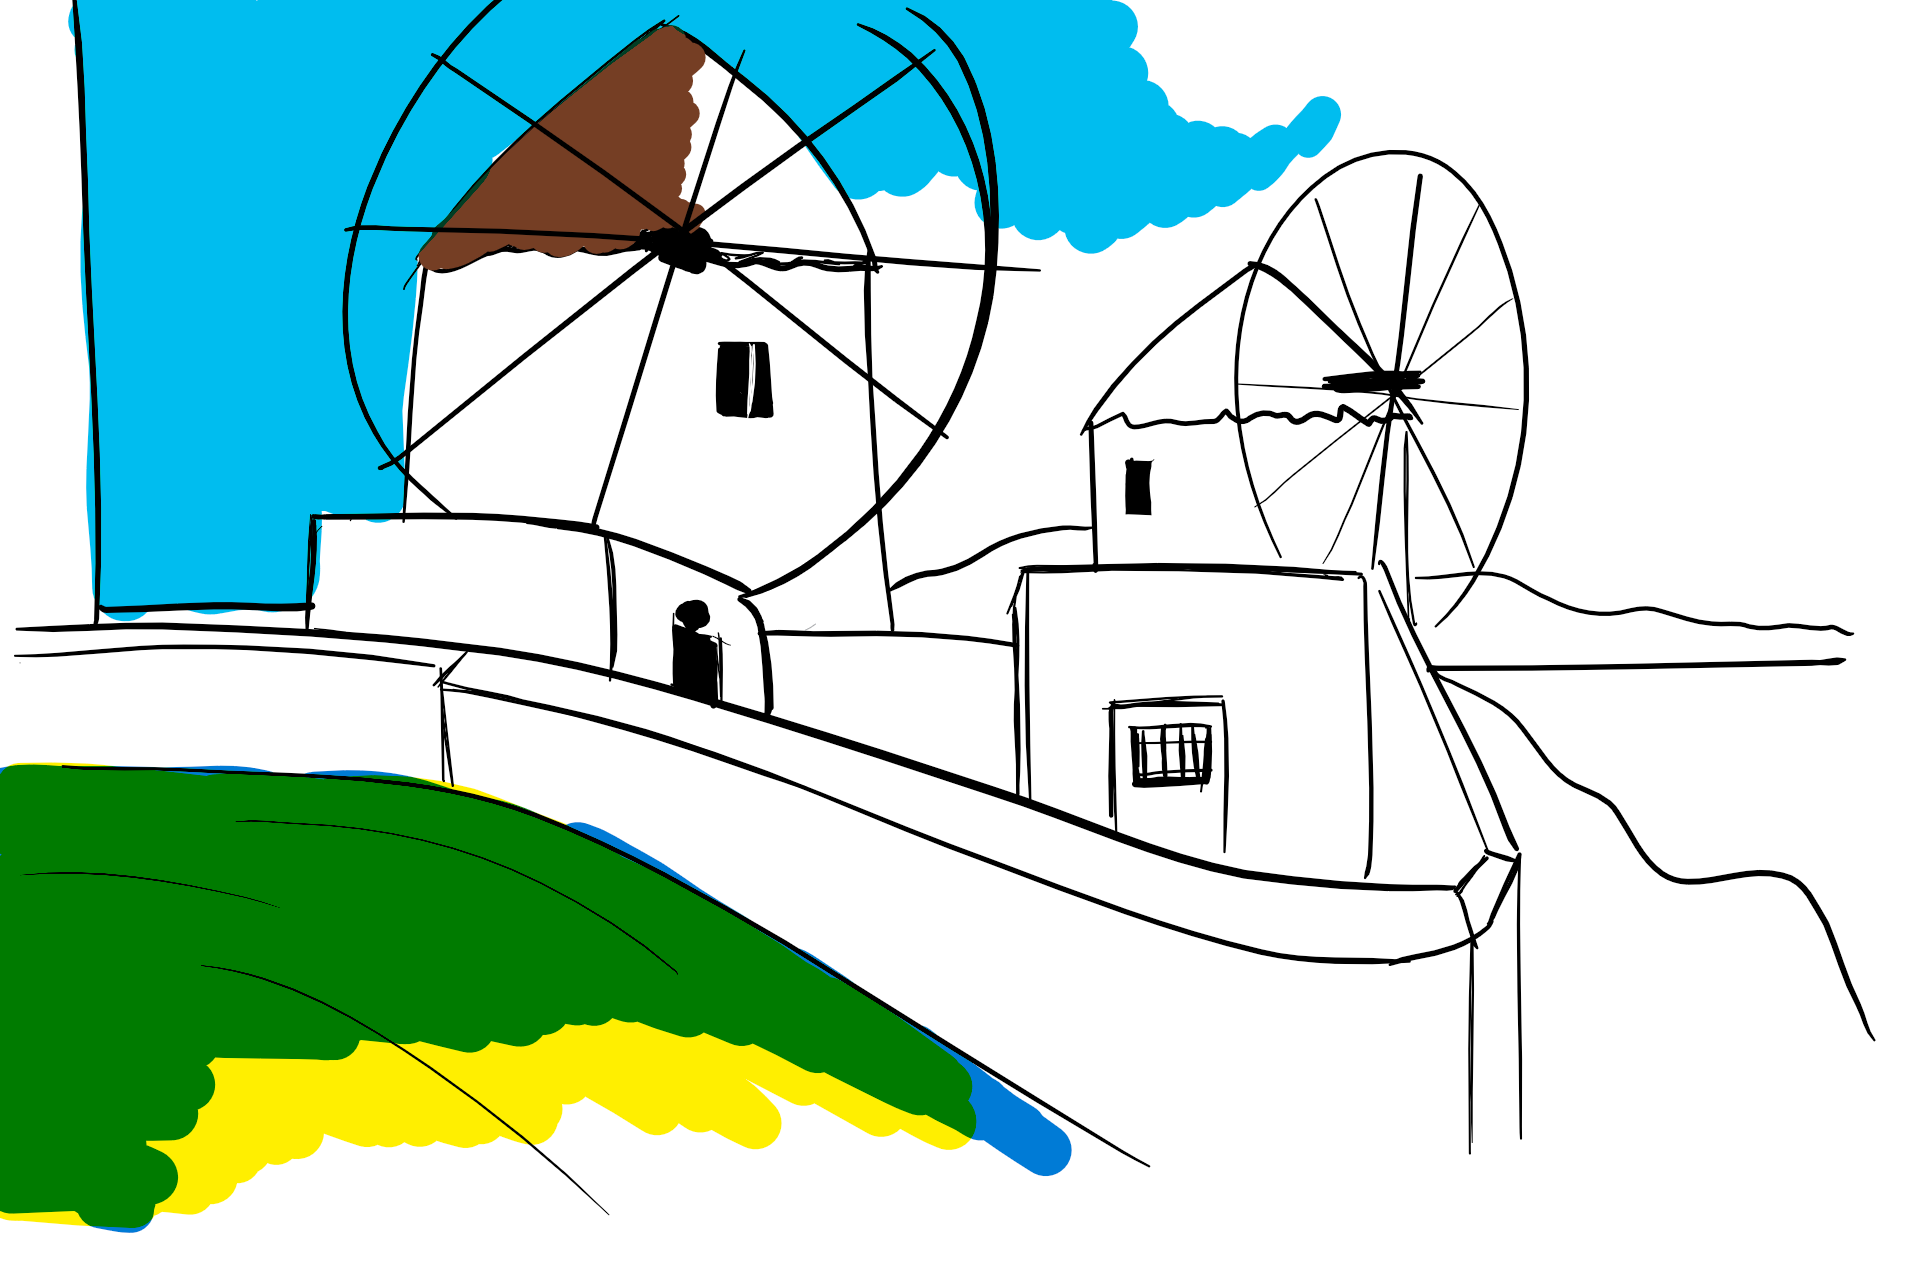
\includegraphics[width=.5\textwidth]{q.png}
\end{figure}}
% Feynman Diagram Setting
\usetikzlibrary{arrows.meta}
\newcommand{\midarrow}{\tikz \draw[-triangle 45] (0,0) -- +(.05,0);}
\tikzset{> = latex, color=blue}
\usetikzlibrary{decorations.markings,decorations.pathreplacing}
\tikzset{
	% style to apply some styles to each segment of a path
	on each segment/.style={draw=blue,
		decorate,
		    decoration={
			show path construction,
			moveto code={},
			lineto code={
				\path [#1]
				(\tikzinputsegmentfirst) -- (\tikzinputsegmentlast);
			},
			curveto code={
				\path [#1] (\tikzinputsegmentfirst)
				.. controls
				(\tikzinputsegmentsupporta) and (\tikzinputsegmentsupportb)
				..
				(\tikzinputsegmentlast);
			},
			closepath code={
				\path [#1]
				(\tikzinputsegmentfirst) -- (\tikzinputsegmentlast);
			},
		},
	},
	% style to add an arrow in the middle of a path
	mid arrow/.style={postaction={decorate,decoration={
				markings,
				mark=at position .55 with {\draw[arrows = {-Latex[width=0pt 7, length=5pt]}] (0pt,.0pt) -- (1.8pt,0pt);}
	}}},
}
\newcommand{\dian}{\tikz{\filldraw[blue](0,0)circle(1pt)}}
\usepackage[compat=1.1.0]{tikz-feynman}
\usepackage{float}
\renewcommand{\normalsize}{\fontsize{8pt}{9.6pt}\selectfont}
\newcommand{\diagsize}{\fontsize{5pt}{6.6pt}\selectfont}